\section{La sustentation et l'aile}

\subsection{Les axes}
\subsubsection{Les 4 forces}
\begin{figure}[H]
		\centering
  		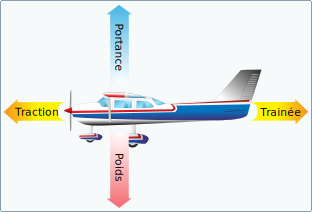
\includegraphics[width=0.8\textwidth]{04-Aerodynamique/img/forces.pdf}
  		\legende{Les 4 forces}{img:forces}	
\end{figure}

\subsection{L'aile}

\subsubsection{Description générale}
Toute aile est composée de plusieurs parties distinctes :
\begin{itemize}
	\item L'\gls{intrados} est la partie inférieure de l'aile. Lorsque l'aile se déplace dans une masse d'air, l'intrados est le siège d'une surpression.
	\item L'\gls{extrados} est la partie supérieure de l'aile. Lorsque l'aile se déplace dans une masse d'air, l'extrados est le siège d'une dépression (l'aile est aspirée vers le haut).
	\item Le \gls{bord d'attaque} \anglais{leading edge} est le point le plus en avant d'un profil d'aile. C'est à ce point que l'air entrera en contact en premier avec l'aile. Il s'agit généralement d'une surface  courbe.
	\item Le \gls{bord de fuite} \anglais{trailing edge} est le point le plus en arrière d'un profil d'aile.  Il s'agit généralement d'une pointe.
\end{itemize}

	\begin{figure}[H]
  	\centering
    \includegraphics[width=0.8\textwidth]{04-Aerodynamique/img/profilAile}
  	\legende{Profil d'une aile}{img:profilAile}
	\end{figure}	
	
	\astuce{Pour se souvenir ou sont situés l'intrados et l'extrados : quand l'avion vol à plat, l'extrados fait face à l'extérieur de la planète, l'intrados regarde vers l'intérieur de la planète.} 
	
\subsubsection{Répartition des pressions autour d'une aile}
	\begin{figure}[H]
		\centering
  		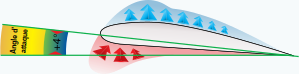
\includegraphics[width=0.8\textwidth]{04-Aerodynamique/img/pressionProfilSelonAngleAttaque4deg.pdf}
  		\legende{La pression autour d'une aile}{img:pressionProfilSelonAngleAttaque}
	\end{figure}	


\subsection{La portance}
\begin{figure}[H]
		\centering
  		\includegraphics[width=0.65\textwidth]{04-Aerodynamique/img/portanceTraineeFinesse_portance.pdf}
  		\legende{Portance en fonction de l'angle d'incidence de l'aile}{img:portanceTraineeFinesse}
	\end{figure}	

\subsubsection{Expression algébrique de la portance}
	\begin{center}
		\huge{$Z = \dfrac{1}{2}\rho S V^2 Cz$}
	\end{center}
	
	avec : \begin{itemize}
	\item $\rho$ : densité de l'air en $kg/m^3$ ($\sim 1,2~kg/m^3$),
	\item $S$ : surface de l'aile en $m^2$,
	\item $V$ : vitesse en $m/s$,
	\item $Cz$ : coefficient de portance (sans unité), valeur liée à la forme de l'aile et à l'incidence.
	\end{itemize}
	

\subsection{La trainée}
\begin{figure}[H]
		\centering
  		\includegraphics[width=0.65\textwidth]{04-Aerodynamique/img/portanceTraineeFinesse_trainee.pdf}
  		\legende{Trainée en fonction de l'angle d'incidence de l'aile}{img:portanceTraineeFinesse}
	\end{figure}	

\subsubsection{Expression algébrique de la trainée}
	\begin{center}
		\huge{$X = \dfrac{1}{2}\rho S V^2 Cx$}
	\end{center}
	
	\begin{itemize}
	\item $\rho$ : densité de l'air en $kg/m^3$ ($\sim 1,2~kg/m^3$),
	\item $S$ : surface de l'aile en $m^2$,
	\item $V$ : vitesse en $m/s$,
	\item $Cx$ : coefficient de trainée (sans unité), valeur liée à la forme de l'aile et à l'incidence.
	\end{itemize}
	
	On constate que l'expression de la portance et de la trainée sont identiques au facteur $Cx$ et $Cz$ près. La portance et la trainée évoluent donc pendant le vol de la même façon.
	
\subsection{Finesse}

\subsection{Polaire d'une aile}
Il est possible de tracer sur un graphique la portance (Cz) en fonction de la trainée (Cx).
\begin{figure}[H]
		\centering
  		\includegraphics[width=0.5\textwidth]{04-Aerodynamique/img/polaireAileMeilleureFinesse.pdf}
  		\legende{Polaire d'une aile, avec point de meilleure finesse}{img:polaireAileMeilleureFinesse}
\end{figure}	

Obtenue en traçant la portance $C_z$ en fonction de la trainée $C_x$. On peut identifier sur cette courbe plusieurs points caractéristiques :
 		\begin{itemize}
 			\item $A$ : $Cz = 0 \Rightarrow$ portance nulle
 			\item $B$ : trainée $C_x$ minimale
 			\item $C$ : $\dfrac{C_z}{C_x}$ minimum $\Rightarrow$ finesse maximale
 			\item $D$ : portance $C_z$ maximale
 			\item $E$ : décrochage
 		\end{itemize}

\subsection{Dispositifs hypersustentateurs et destructeurs de portance}
	\subsubsection{Dispositifs hypersustentateurs}
	Lors des phases d'atterrissage et de décollage, il est souhaitable de pouvoir évoluer à la vitesse la plus faible possible.	On peut obtenir cela grâce à une plus grande surface d'aile, ou concevoir l'aile pour augmenter son $Cz$. Mais, comme on l'a vu, toute augmentation du coefficient de portance ou de la surface de l'aile se fait au prix d'une augmentation de la trainée, indésirable en croisière (réduction des performances de montée, de vitesse maximale, augmentation de la consommation...).
	
	La solution consiste à modifier ces 2 paramètres (surface, $Cs$) uniquement quand on souhaite pouvoir voler moins vite. Cela est obtenu grâce aux dispositifs hypersustentateurs, qui sont de 2 types : \begin{itemize}
	\item volets \anglais{flaps}, situés sur ou à proximité du bord de fuite,
	\item becs \anglais{slats}, situés sur le bord d'attaque.
	\end{itemize}
	
	Ces dispositifs sont actionnés (par l'équipage, ou dans certains cas, automatiquement) pour le décollage, sont rentrés durant la montée, puis sont ressortis en vue de l'atterrissage. Sur la plupart des appareils, il est possible de sélectionner plusieurs "niveaux" de sortie de ces dispositifs. Ils sont généralement sortis de façon plus importante pour l'atterrissage, phase ou l'augmentation de la trainée est moins problématique (au décollage, la trainée grève les performances de montée).
	
	La commande est transmise à ces surfaces par un jeu de tringles, ou sont motorisés par des systèmes électriques ou hydrauliques. \\
	
	\definition{Lorsqu'un appareil a tous ses dispositifs hypersustentateurs rentrés, on dit qu'il est en  \textbf{\gls{configuration lisse}}.}
	
		\paragraph{\Gls{volet}s}
			\subparagraph{Volets de courbure}
			Le type le plus simple sont les volets de courbure. Ces volets modifient le profil de l'aile en augmentant la courbure de l'aile à proximité du bord de fuite. Ces volets augmentent sensiblement le coefficient de portance, mais aussi la trainée.
		\begin{figure}[H]
			\centering
  			\includegraphics[width=0.4\textwidth]{04-Aerodynamique/img/hypersustentateurs/voletsDeCourbure.pdf}
  			\legende{Volets de courbure}{img:voletsDeCourbure}	
		\end{figure}
		
			\subparagraph{Volets d'intrados}
		Les volets d'intrados sont moins fréquemment utilisés sur les avions modernes. Ils augmentent la portance mais également la trainée dans des proportions très importantes. Ce type de volet est souvent assimilé à des aérofreins. 
		\begin{figure}[H]
			\centering
  			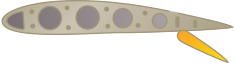
\includegraphics[width=0.4\textwidth]{04-Aerodynamique/img/hypersustentateurs/voletDIntrados.pdf}
  			\legende{Volets d'intrados}{img:voletDIntrados}	
		\end{figure}
		
			\subparagraph{Volets à fente}
			Le volet à fente se déploie sur le bord de fuite. Il augmente donc la portance en modifiant la surface de l'aile.
		\begin{figure}[H]
			\centering
  			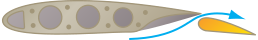
\includegraphics[width=0.4\textwidth]{04-Aerodynamique/img/hypersustentateurs/voletFowler.pdf}
  			\legende{Volets Fowler}{img:voletFowler}	
		\end{figure}
		
			\subparagraph{Volets Fowler}
			Le volet Fowler (du nom de son inventeur américain Harlan Fowler) combine le volet à fente et le volet de cambrure. Il se déploie sur le bord de fuite puis s'abaisse vers le bas. Il augmente donc la portance en modifiant la surface de l'aile puis la cambrure (donc le $Cz$).
		
		\begin{figure}[H]
			\centering
  			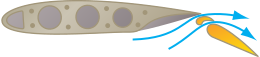
\includegraphics[width=0.4\textwidth]{04-Aerodynamique/img/hypersustentateurs/voletFowlerAFente.pdf}
  			\legende{Volets Fowler}{img:voletFowlerAFente}	
		\end{figure}
		
		\paragraph{\Gls{bec}s}
		Les becs de bord d'attaque sont des surfaces qui sortent à l'avant de l'aile. Ils augmente la surface de l'aile.
		\begin{figure}[H]
			\centering
  			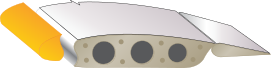
\includegraphics[width=0.4\textwidth]{04-Aerodynamique/img/hypersustentateurs/becs.pdf}
  			\legende{Bacs de bord d'attaque}{img:becs}	
		\end{figure}
		
	\subsubsection{Les aérofreins}
	Les aérofreins \anglais{air brakes} sont des dispositifs situés sur les ailes ou sur le fuselage et dont l'objectif est d'augmenter la trainée. Ils permettent d'augmenter le taux de descente sans augmenter la vitesse.
	
	Les aérofreins sont généralement installés sur les avions de ligne, les planeurs ou encore les navettes spatiales.
	
	\begin{figure}[H]
	\begin{minipage}[c]{0.5\linewidth}
	\includegraphics[width=\linewidth]{01-EtudeAeronefs/img/afPlaneur.jpg}
	\legende{Planeur avec aérofreins de voilure déployés}{img:afPlaneur}
	\end{minipage}
	\hfill
	\begin{minipage}[c]{0.5\linewidth}
	\includegraphics[width=\linewidth]{01-EtudeAeronefs/img/afBae146.jpg}
	\legende{Aérofreins de cône de queue déployés}{img:afBae146}
	\end{minipage}
	\end{figure}
		
	\subsubsection{Dispositifs destructeurs de portance}
	Les dispositifs destructeurs de portance \anglais{spoilers} annulent totalement la portance et augmentent de façon importante la trainée.
	
	Ils sont généralement utilisés à l'atterrissage sur les avions de ligne pour plaquer l'aéronef au sol, et donc augmenter le poids supporté par le train d'atterrissage, ce qui augmente l'adhérence et donc l'efficacité du freinage.
	
	\begin{figure}[H]
	\centering
	\includegraphics[width=0.5\linewidth]{01-EtudeAeronefs/img/spoilerA320.jpg}
	\legende{A320 avec spoilers déployés}{img:spoilerA320}
	\end{figure}
	